\documentclass[aspectratio=169]{beamer}
\usepackage[backend=biber,style=ieee]{biblatex}
\addbibresource{references.bib}
\renewcommand*{\bibfont}{\tiny}
\setbeamertemplate{bibliography item}{\insertbiblabel}

%\usepackage[sfdefault]{universalis}
%\usepackage[T1]{fontenc}
%\renewcommand{\sfdefault}{cmss}
\renewcommand{\familydefault}{\sfdefault}
%\usepackage{fontspec}
%\setmainfont{Utopia}

\usetheme[width=3.5cm]{Hannover}
\usecolortheme{beaver}
\usepackage{geometry}
\usepackage{multicol}
\usepackage{parskip}
\usepackage{color}
\usepackage{url}
\usepackage{hyperref}
\usepackage{listings}
\usepackage[ruled, vlined,commentsnumbered]{algorithm2e}
%\usepackage{algorithmicx}
%\usepackage{algpseudocode}
%\usepackage{algorithm}
\usepackage{graphicx}
\usepackage[nonumberlist,style=long]{glossaries}
\setlength{\parindent}{0pt}
\setlength{\parskip}{10pt plus3pt minus3pt}

\DeclareGraphicsRule{*}{mps}{*}{}
\definecolor{dkgreen}{rgb}{0,0.6,0}
\definecolor{gray}{rgb}{0.5,0.5,0.5}
\definecolor{mauve}{rgb}{0.58,0,0.82}
 
\lstset{ %
  language=Python,                % the language of the code
  basicstyle=\footnotesize,           % the size of the fonts that are used for the code
  numbers=left,                   % where to put the line-numbers
  numberstyle=\tiny\color{gray},  % the style that is used for the line-numbers
  stepnumber=2,                   % the step between two line-numbers. If it's 1, each line 
                                  % will be numbered
  numbersep=5pt,                  % how far the line-numbers are from the code
  backgroundcolor=\color{white},      % choose the background color. You must add \usepackage{color}
  showspaces=false,               % show spaces adding particular underscores
  showstringspaces=false,         % underline spaces within strings
  showtabs=false,                 % show tabs within strings adding particular underscores
  frame=single,                   % adds a frame around the code
  rulecolor=\color{black},        % if not set, the frame-color may be changed on line-breaks within not-black text (e.g. commens (green here))
  tabsize=2,                      % sets default tabsize to 2 spaces
  captionpos=b,                   % sets the caption-position to bottom
  breaklines=true,                % sets automatic line breaking
  breakatwhitespace=false,        % sets if automatic breaks should only happen at whitespace
  title=\lstname,                   % show the filename of files included with \lstinputlisting;
                                  % also try caption instead of title
  keywordstyle=\color{blue},          % keyword style
  commentstyle=\color{dkgreen},       % comment style
  stringstyle=\color{mauve},         % string literal style
  escapeinside={\%*}{*)},            % if you want to add LaTeX within your code
  morekeywords={*,...}               % if you want to add more keywords to the set
}

\hypersetup{
%    pdfstartview=FitB,     % Fit width
    colorlinks=true,       % false: boxed links; true: colored links
    linkcolor=red,          % color of internal links
    citecolor=red,        % color of links to bibliography
    filecolor=magenta,      % color of file links
    urlcolor=blue           % color of external links
}

\defbeamertemplate*{title page}{customized}[1][]
{
	\usebeamerfont{title}\inserttitle\par
	\usebeamerfont{subtitle}{\usebeamercolor[fg]{subtitle}\insertsubtitle\par}
	\bigskip 
	\usebeamerfont{author}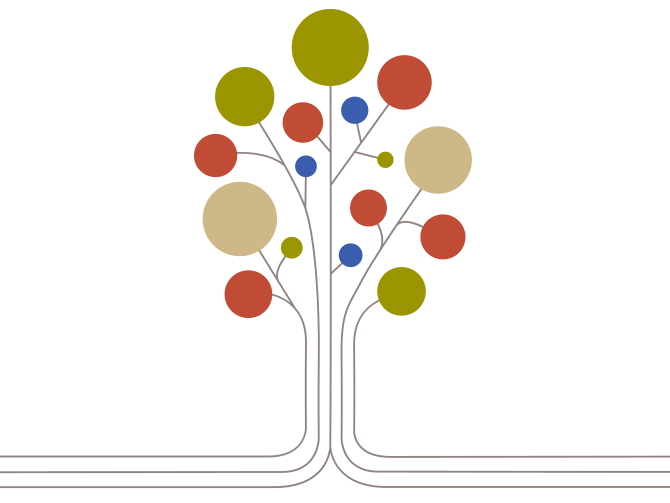
\includegraphics[scale=0.1]{acumed.png}\par\insertauthor\par
	\usebeamerfont{institute}\insertinstitute\par
	\usebeamerfont{date}\insertdate\par
	\usebeamercolor[fg]{titlegraphic}\inserttitlegraphic
}
\defbeamertemplate*{part page}{customized}[1][]
{
	\renewcommand{\partname}{Day}
	\begingroup
	\centering
	{\usebeamerfont{part name}\usebeamercolor[fg]{part name}\partname~\insertromanpartnumber}
	\vskip1em\par
	\begin{beamercolorbox}[sep=16pt,center,#1]{part title}
		\usebeamerfont{part title}\insertpart\par
	\end{beamercolorbox}
	\endgroup
}
\setbeamercolor{section in sidebar}{fg=black}
\setbeamertemplate{itemize items}[ball]
\setbeamertemplate{enumerate items}[ball]
\AtBeginPart{\frame{\partpage}}

\author{Peter Tillotson}
\institute{Acumed Consulting}
\title{Anomaly Detection}
\subtitle{Day 1: What is an anomaly? How do we spot them?\newline 
Day 2: Machine learning, clustering and classification\newline
Day 3: Periodicity, and an entity centric view 
}

\begin{document}
\frame{\titlepage}


\part{What is an anomaly? How do we spot them?}
\begin{frame}
	\frametitle{Table of Contents}
	\tableofcontents[hideallsubsections]
	%\tableofcontents[currentsection]
\end{frame}

\section{Module Aims}
\begin{frame}
\frametitle{What we'll learn}
By the end of today, we will have: 
\begin{itemize}
\item a good understanding of anomaly detection
\item discussed in detail a number of techniques commonly used to detect anomalies
	\begin{itemize}
	\item linear regression
	\item classification 
	\item clustering
	\end{itemize}
\item introduced Python Panda's and
\item implemented a linear regression model in with Panda's
\end{itemize} 
\end{frame}

\begin{frame}
\frametitle{Prerequisites}
\begin{tabular}{|p{8cm} | l|}
\hline
{{\bf Programming:} basic understanding of programming concepts including:
	\begin{itemize}
		\item flow control
		\item functions
		\item data structures
		\item types (int, float)
	\end{itemize}} & Good \\ \hline
{\bf Python:} be familiar with the Python & Some \\ \hline
{\bf Math:} basic statistics (mean, variance) & Some \\
\hline
\end{tabular}
\end{frame}

\section{Overview}
\subsection{What is Anomaly Detection?}
\begin{frame}
\frametitle{Definition: Anomaly}
\href{http://www.oxforddictionaries.com/definition/english/anomaly}{Anomaly} from the Oxford Dictionary:
\begin{quote}
	Something that deviates from what is standard, normal, or expected
\end{quote}
But that includes 5$\%$ of all data so what we're really interested in are events that 
are particularly odd or inherently risky. Ideally something that is actionable and that 
probably needs human intervention.

We want to avoid false positives, though whilst potentially rare these create noise and reduce an analysts trust of an automated solution. 

We also want to avoid false negatives, real risks that we failed to spot.  
\end{frame}

\subsection{What is normal?}
\begin{frame}[fragile]
\frametitle{Some code}
\begin{lstlisting}
import json
def my_function():
	m_str = json.dumps({'name': 'peter', 'msg':'dont it look nice'})
	print 
my_function()
\end{lstlisting}
\cite{data:yahoo}
\end{frame}

\subsection{What methods are used?}
\subsubsection{Linear regression}
\subsubsection{Classification}
\subsubsection{Clustering}


\section{Python Pandas}
\subsection{Data structures}
\subsubsection{Sequences}
\subsubsection{DataFrames}
\subsection{IO: loading and writing data}
\subsection{Plotting graphs}

\section{Linear Regression}
More often than not, time series data are `non-stationary'; that is, the values of the time series do not fluctuate around a constant mean or with a constant variance.
\section{Exercise 1: Anomaly detection by linear regression in Pandas}

\part{Machine learning, clustering and classification}

\part{Periodicity, and an entity centric view}

\begin{frame}
\frametitle{What is Periodicity}
Anything that repeats with a fixed interval can be said to periodic. If you can
be guruanteed delivery of your signal, and have a trusted source for timestamps 
then it is possible to run Descrete Fourier Transforms and get a frequency domain 
representation of your signal.   

Often this is not possible and the following approaches can be used to to handle trends
and seasonality in data. 
\begin{itemize}
\item Curve fitting - STL / Decomposition
\item Twitter's Seasonal Hybrid ESD \cite{ref:twitter-blog}
\begin{itemize}
    \item Time series decomposition
    \item Generalised ESD
\end{itemize}
\item Numenta's Hierarchical Temporal Memory \cite{ref:numenta-whitepaper}
\end{itemize} 

\end{frame}

\begin{frame}[allowframebreaks]
\frametitle{Generalized ESD (extreme Studentized deviate)}
The Generalized ESD\cite{ref:rosner} test is defined for the two hypothesis:\newline
$H_0$\hspace{24pt}There are no outliers in the data set\newline
$H_r$\hspace{24pt}There are up to $r$ outliers in the data set\newline
Compute:\newline
\begin{equation}
R_i=\frac{\max_i | x_i - \mu | }{\sigma}
\end{equation}
with $\mu$ and $\sigma$ denoting the mean and standard deviation, respectively.

Remove the observation that maximizes $| x_i - \mu |$ and then recompute the above statistic with $n - 1$ observations. Repeat this process until $r$ observations have been removed. This results in the $r$ test statistics $R_1, R_2, \ldots, R_r$.

Corresponding to the r test statistics, compute the following $r$ critical values:\newline
\begin{equation}
\lambda_i=\frac{ (n-1)t_{p,n-i-1}}{\sqrt{(n-i-1 + t^2_{p, n-i-1})(n-i+1)}}  
\end{equation}
for $i=1,2,\ldots,r$

where $t_{p,v}$ is the $100p$ percentage point from the $t$ distribution with $v$ degrees of freedom and
\begin{align*}
p = 1 - \frac{\alpha}{2(n-i+1)}
\end{align*}
The number of outliers is the largest $i$ such that $R_i > λ_i$.
\end{frame}
\AtBeginPart{}
\part{R{\small EFERENCES}}
\begin{frame}
	\centering
	\vskip1em\par
	\begin{beamercolorbox}[sep=16pt,center]{part title}
		\usebeamerfont{part title}\insertpart\par
	\end{beamercolorbox}
\end{frame}

\begin{multicols*}{2}[\frametitle{} \usebeamertemplate{frametitle}]
	\printbibliography
\end{multicols*}

%\begin{frame}[allowframebreaks]
%	\frametitle{References}
%	\bibliographystyle{amsplain}
%	\bibliography{./references}
%\end{frame}
\end{document}